
\section{EG6 experimental setup}
The experiment described in this note has been carried out in the Hall B of 
the Thomas Jefferson National Accelerator Facility (JLab), Virginia, USA. Hall 
B houses the CEBAF Large Acceptance Spectrometer (CLAS). Our experiment was 
performed in 2009 with a longitudinally-polarized electron beam of 6.064 GeV 
scattering onto a 6 $atm$ gaseous $^{4}He$ target to study the nuclear medium 
modifications of parton distributions using the DVCS off the target. 

\subsection{CLAS detector} To ensure the exclusivity of our reaction, the basic 
setup of CLAS was upgraded with a Radial Time Projection Chamber (RTPC) to 
detect the low-energy recoil nuclei, an additional calorimeter (IC) to 
detect the energetic forward-emitted real photons and a solenoid magnet to 
minimize the effects of M\o ller electrons. In the following subsections, we rapidly 
present the sub-detectors previously used by the collaboration,
the RTPC design and calibration are detailed in the next chapter.

\subsection{Inner calorimeter}
In the basic setup of CLAS, the photons are detected by the forward 
electromagnetic calorimeters (EC) which cover polar angles from 8$^{\circ}$ to 
45$^{\circ}$. With a 6 GeV electron beam, a large part of the DVCS photons are 
produced at polar angles below 15$^{\circ}$, where the acceptance of the EC
is small. In the CLAS-E1DVCS experiment (2005), CLAS was upgraded with the 
addition of an Inner Calorimeter (IC). This calorimeter covers completely the 
polar angles between 5$^{\circ}$ and 15$^{\circ}$. Figure \ref{fig:CLAS_RTPC_2} 
shows a schematic plot of our experimental setup. The front face of the IC is 
facing the downstream side of the Radial TPC (RTPC) and placed at 16 cm from 
the center of CLAS.

\begin{figure}[tp]
\centering
%\vspace{-0.28in}
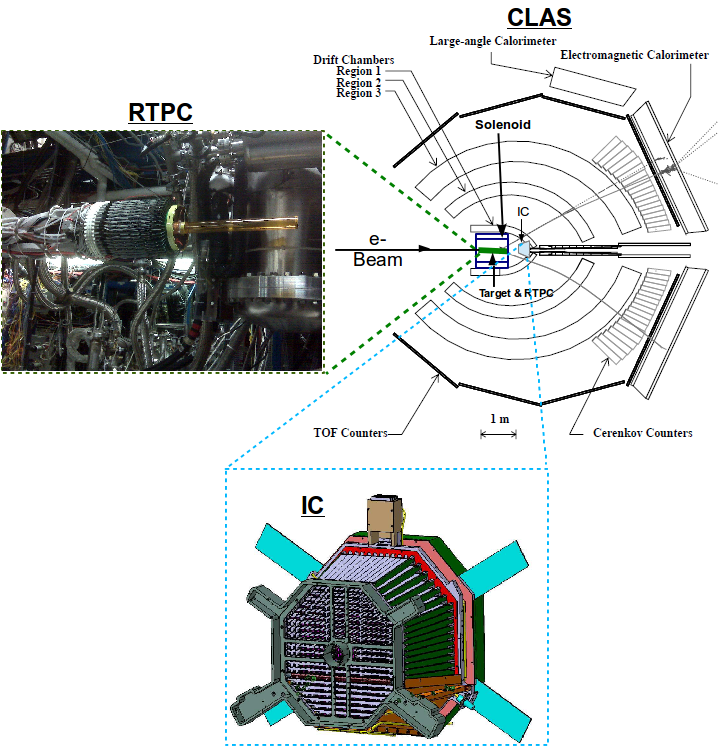
\includegraphics[scale=0.54]{fig/clas_rtpc_3.png}
\caption{The CLAS-EG6 experimental setup in the y-z plane. The basic apparatus of CLAS is shown in the right top plot, a zoom on the IC is shown on the bottom plot, and a photo of the RTPC and the target are shown in the left top plot. The RTPC is surrounded by a solenoid (in blue).} 
\label{fig:CLAS_RTPC_2}
\end{figure} 

The IC is constructed from 424 lead-tungstate (PbWO$_{4}$) crystals. Each 
crystal is 16 cm long (corresponding to 17 radiation lengths) with a 
1.33~$\times$~1.33 cm$^2$ front surface and a 1.6~$\times$~1.6 cm$^2$ back 
surface. The energy resolution is around 3 to 4$\%$ for photon energies between 
2 GeV and 5 GeV and the angular resolution is between 3 to 5 mrad for the same 
energy range \cite{Hyon-suk}.

\subsection{Solenoid}
At occupancies greater than 4$\%$, the efficiency of the drift chambers 
starts to drop and the resolution gets worse. The first region of the DCs (R1) 
has a higher occupancy than the other two regions (R2 and R3), mostly due to 
noise. This noise mainly comes from the M\o ller electrons, which are 
low-energy electrons produced in the scattering of the electron beam on the 
target's electrons. To reduce the effect of the noise, CLAS was upgraded by 
adding a solenoid that surrounds the target. The magnet provides a nominal 
field of 4.5 T at the center of the target. This solenoid deflects the produced 
M\o ller electrons to very forward angles preventing them from arriving to the 
drift chamber, the IC or the RTPC. Figure \ref{fig:solenoid} shows a GEANT3 simulation of the 
M\o ller electrons tracks without applying the solenoid field (left), and how 
these electrons are bent to low polar angles, less than 4$^{\circ}$, when the 
solenoid field is applied.

 
\begin{figure}[tp]
\centering
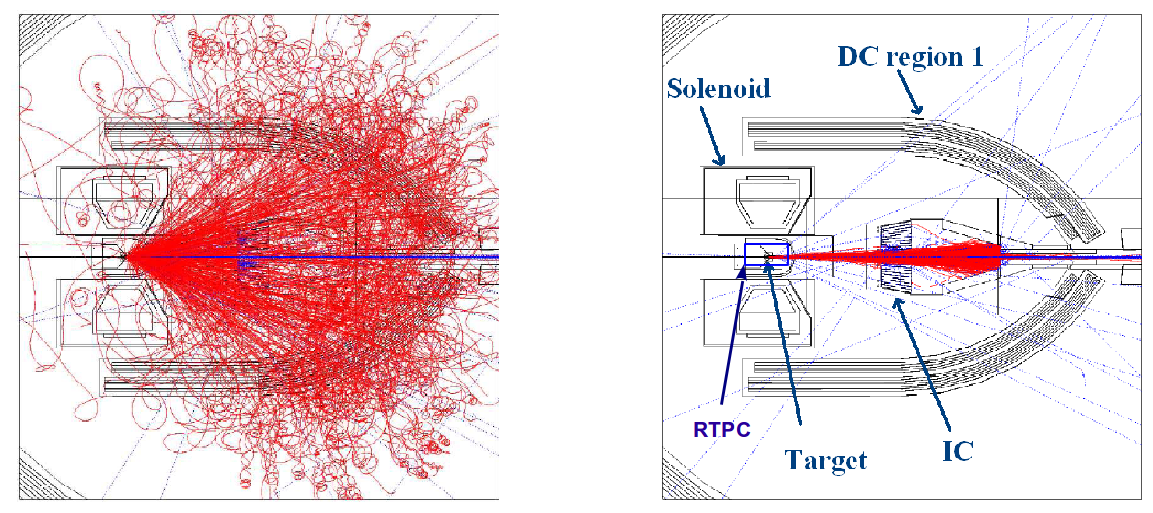
\includegraphics[scale=0.36]{fig/solenoid.png}
\caption{The tracks of the produced M\o ller electrons (in red) without 
applying the solenoid field (left) and with it (right) 
\cite{Hyon-suk}. } \label{fig:solenoid}
\end{figure}

\subsection{Run conditions}

Table \ref{table:eg6_char} summarizes the different beam energies used during 
the experimental run CLAS-EG6 with the details about the beam, the torus, and 
the solenoid currents.  

\begin{table}[!h]
   \centering
   \begin{center}
      \begin{tabular}{|l|l|l|l|}
         \hline
         beam energy [GeV] & Beam current [nA] & Torus current [A] & Solenoid 
         current [A] \\ \hline
         1.204 & 150 & 2100 & 450 \\
         \hline
         5.7  & 100 & 1900 & 450 \\
         \hline
         6.064 & 120-150 & 2100 & 450\\
         \hline
         1.269  & 100 & 1900 & 450\\
         \hline
      \end{tabular}
      \caption{The different beam energies used during the experimental run 
      period CLAS-EG6 with the currents in the beam, torus, and the solenoid. }
      \label{table:eg6_char}
   \end{center}
\end{table}

